\documentclass[12pt, a4paper]{report}
\usepackage{geometry}
\usepackage{graphicx}
\usepackage{float}
\usepackage{subfigure}
\usepackage{booktabs}
\usepackage{appendix}
\geometry{left=2cm,right=2cm}
\title{COVID-19 and Economics Indicators in the UK}
\author{Siyu YANG}
\date{}

\begin{document}
\maketitle

\section{Research Questions}
This report is aimed to research on the associations between the severity of COVID-19 and some important 
economics indicators in the UK. More specifically, this report will answer the following questions:
1) Which COVID-19 severity indicator(s) and which economics indicator(s) have high and significant relationships?
2) And how the severity indicator(s) impact the economics indicator(s) exactly?


\section{Datasets}
\subsection{COVID-19 Datasets (updated on 05-02-2021)}
The following three COVID-19 datasets contain the number of positive cases, deaths, and patients admitted to hospitals, 
respectively. Each dataset includes the newly-add number and cumulative number.\par
\noindent
1) Positive cases by spicemen date
\footnote[1]{https://coronavirus.data.gov.uk/details/cases};\par
\noindent
2) Deaths with COVID-19 within 28 days of positive test by date of death
\footnote[2]{https://coronavirus.data.gov.uk/details/deaths};\par
\noindent
3) Patients admitted to hospital
\footnote[3]{https://coronavirus.data.gov.uk/details/healthcare}\par
\begin{figure}[H]
\centering
    \subfigure[COVID19 Cases]{
    \label{Fig.sub.1}
    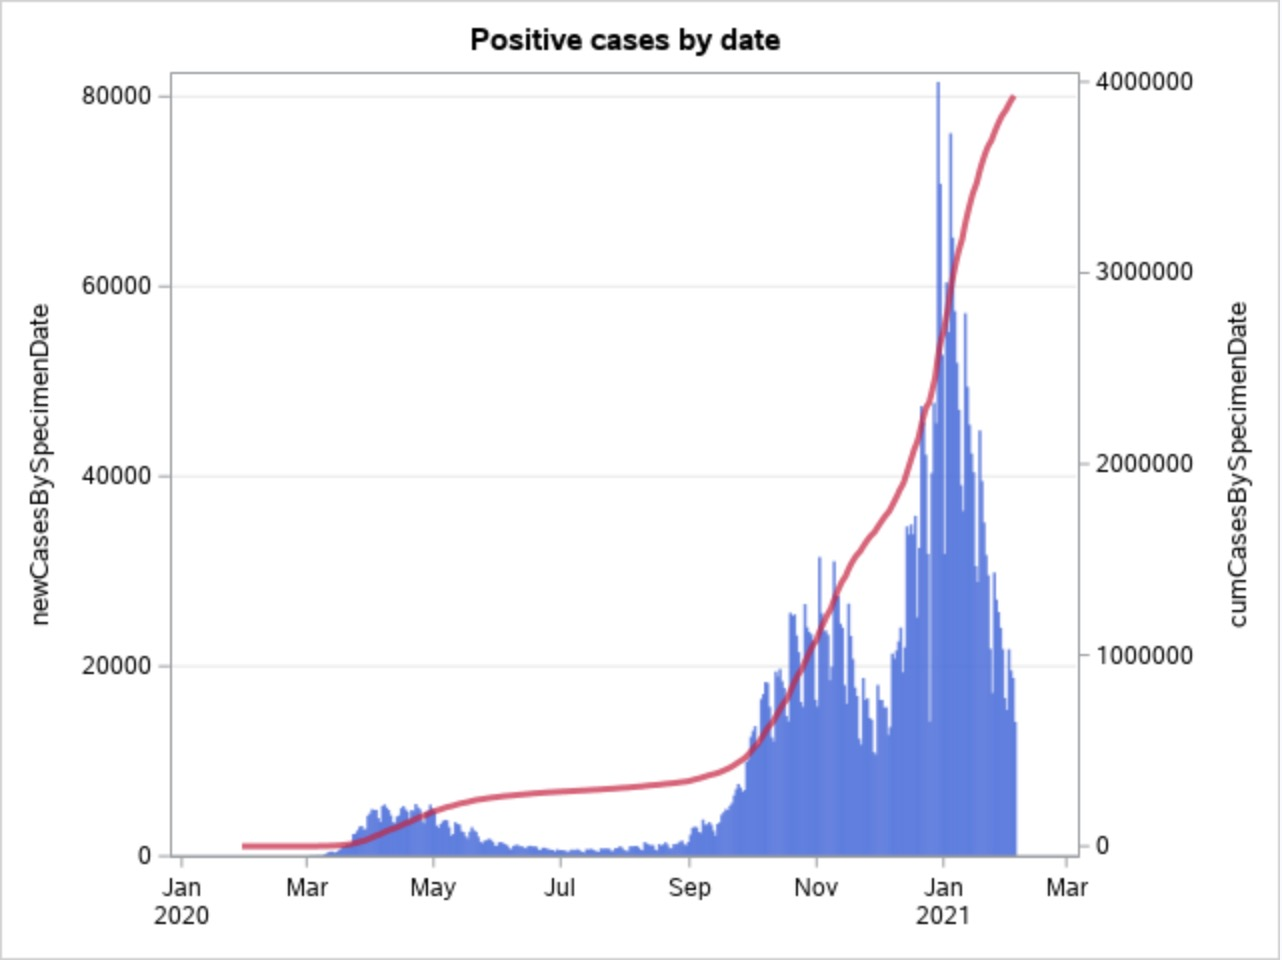
\includegraphics[width=5cm]{covid-19_cases.jpg}}
    \subfigure[COVID19 Deaths]{
    \label{Fig.sub.2}
    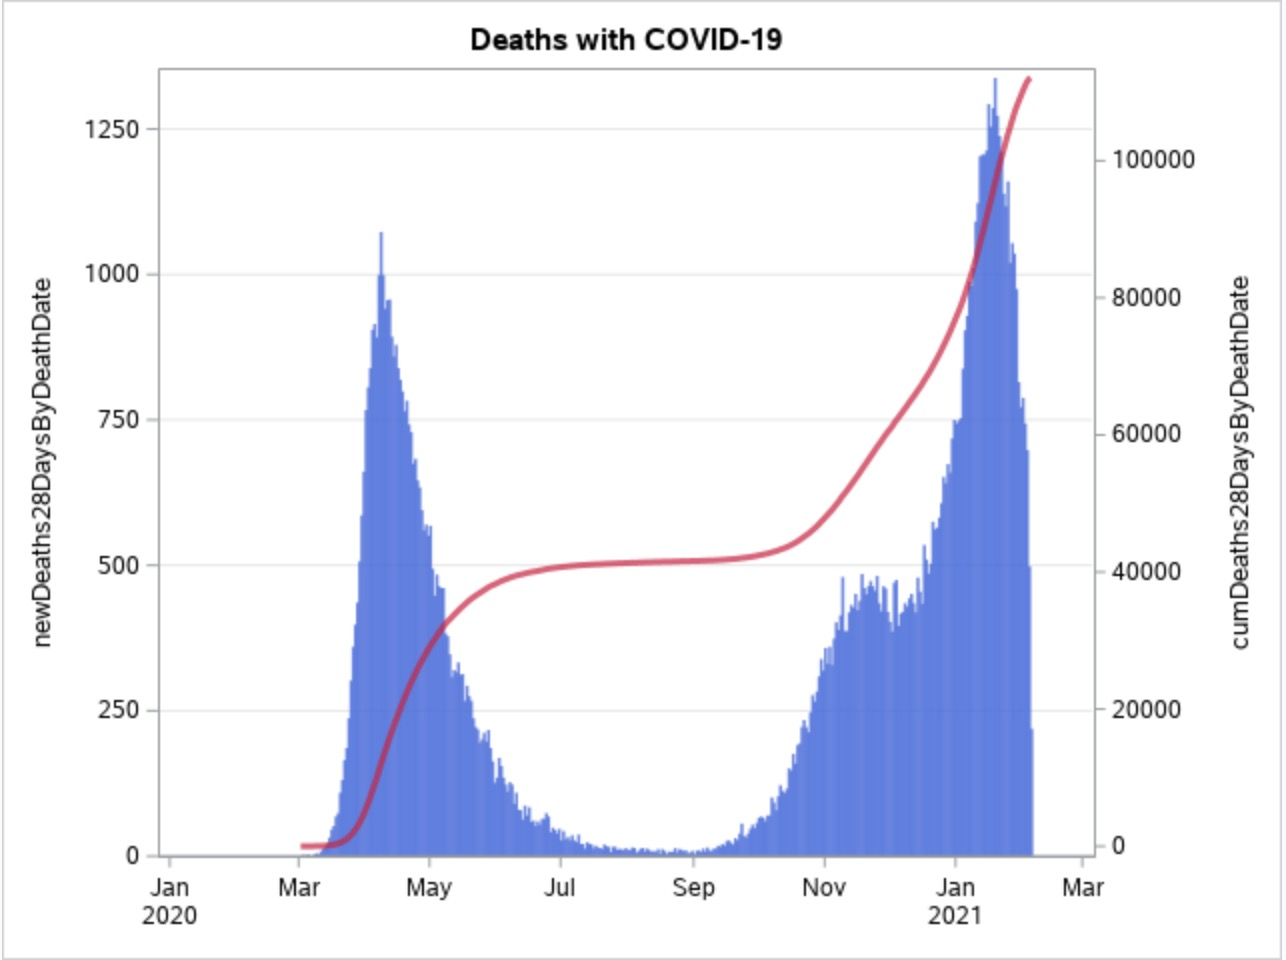
\includegraphics[width=5cm]{covid19_deaths.jpg}}
    \subfigure[COVID19 Patients]{
    \label{Fig.sub.3}
    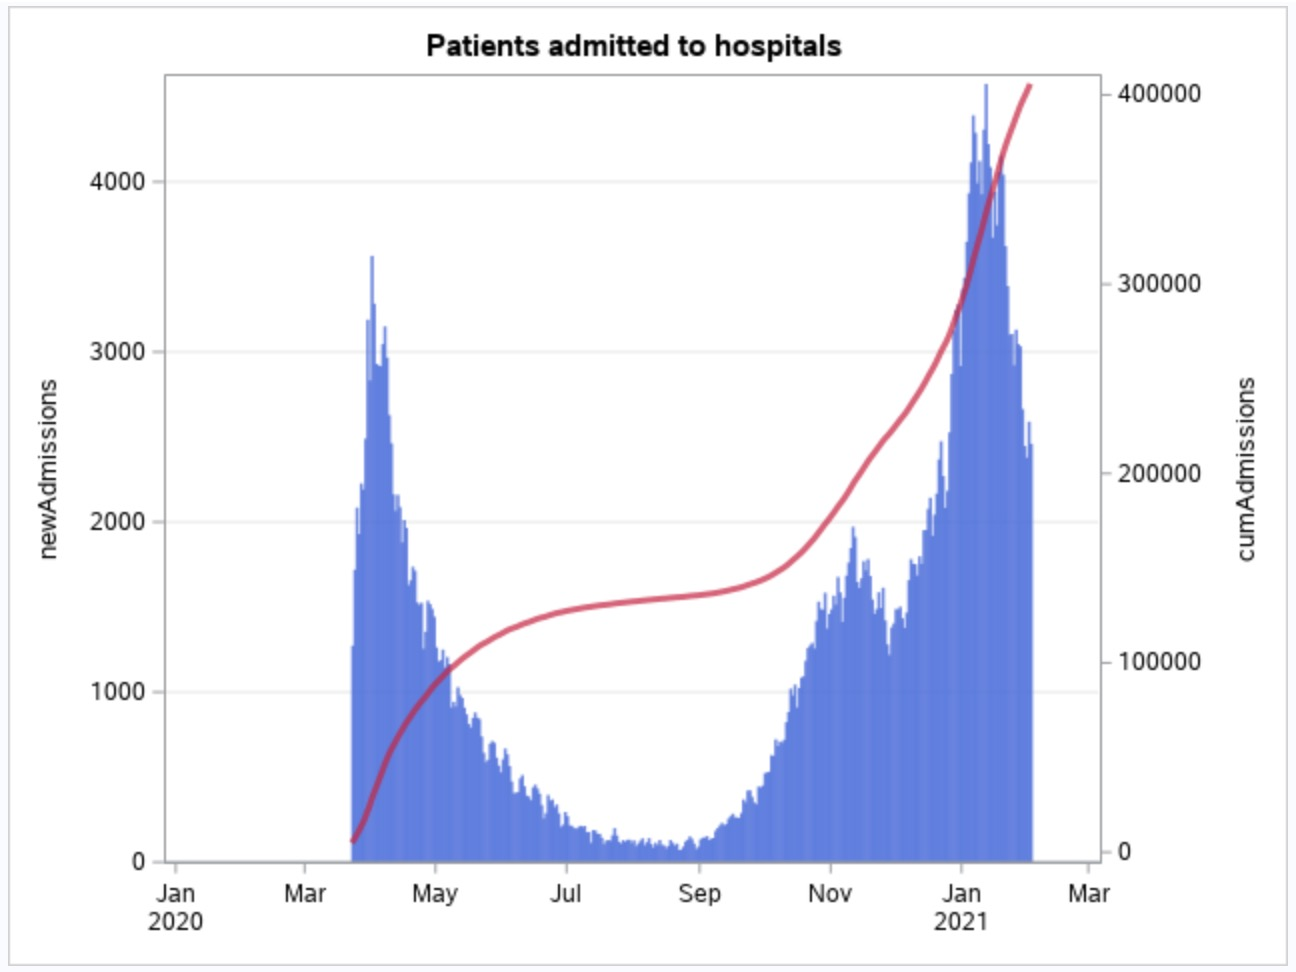
\includegraphics[width=5cm]{covid19_patients.jpg}}
    \caption{COVID19 Indicators}
    \label{Fig.main}
\end{figure}

\subsection{Economic indicators (updated in November 2020)} 
The following two datasets contain the data of five economics indicators: monthly GDP, service index, 
production index, construction index, and unemployment rate.\par
\noindent
1) Monthly GDP and components index (seasonally adjusted)
\footnote[4]{https://www.ons.gov.uk/economy/grossdomesticproductgdp/};\par
\noindent
2) Unemployment rate (aged 16 and over, seasonally adjusted)
\footnote[5]{https://www.ons.gov.uk/employmentandlabourmarket/peoplenotinwork/unemployment/}
\begin{figure}[H] 
\centering 
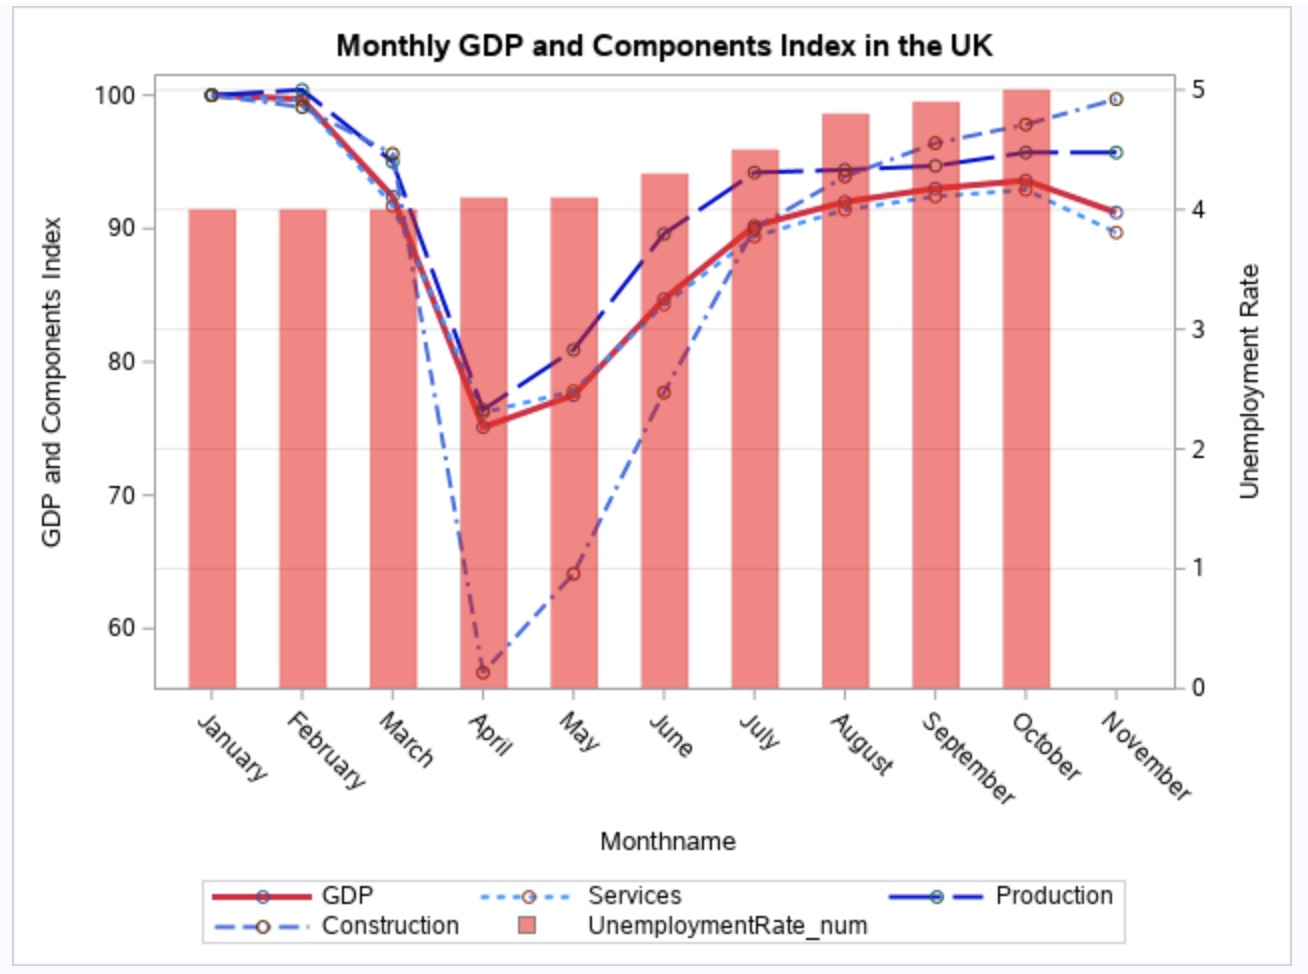
\includegraphics[width=9cm]{economics.jpg} 
\caption{Economics Indicators}
\end{figure}
    
\subsection{Stock Index (updated on 05-02-2021)}
1) FTSE 100 Index;\par
\noindent
2) FTSE All-Share Index
\footnote[6]{Source: Capital IQ}
\begin{figure}[H] 
\centering 
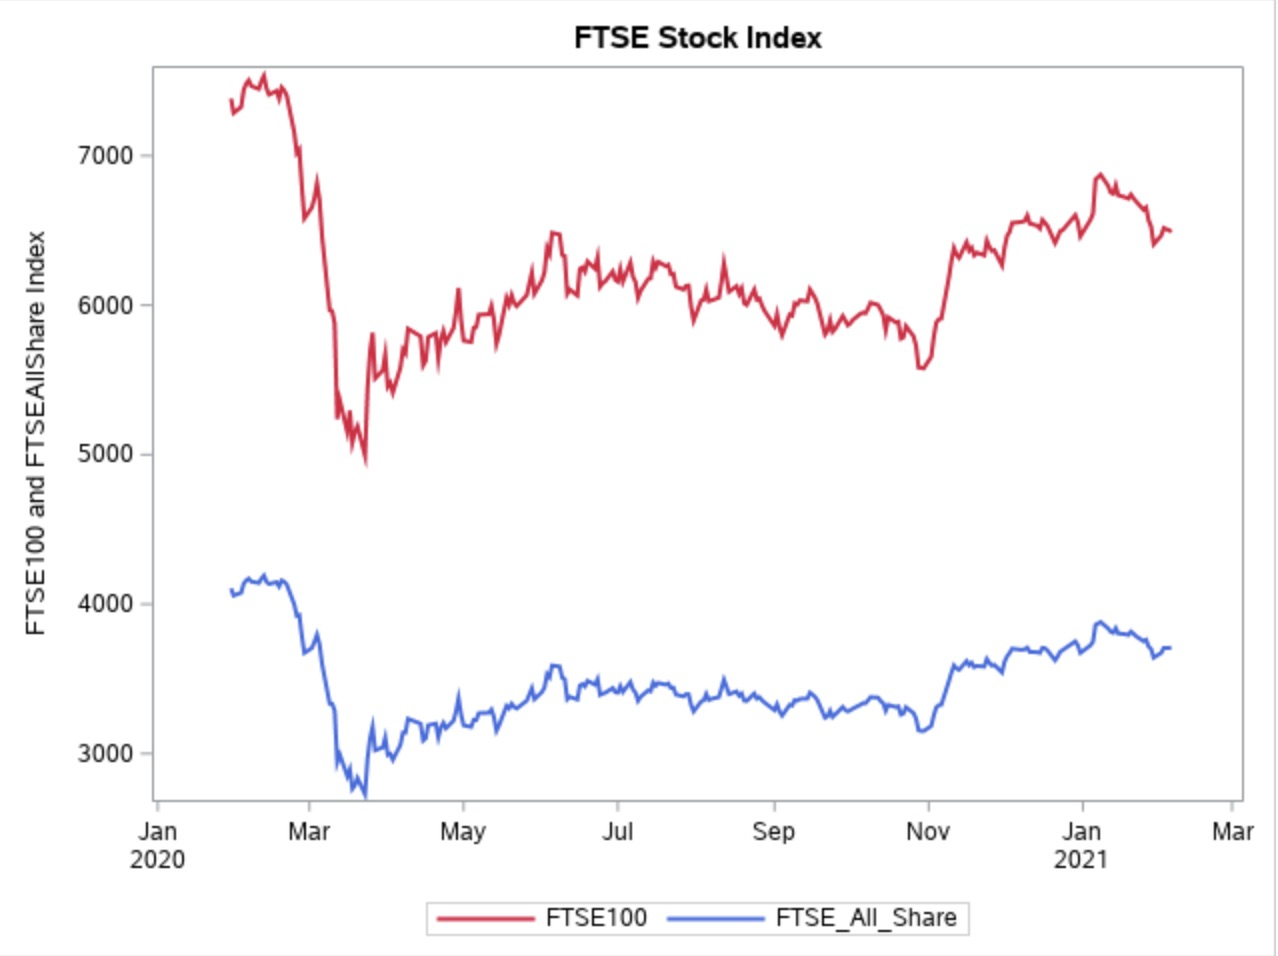
\includegraphics[width=9cm]{ftse.jpg} 
\caption{FTSE Stock Indicators}
\end{figure}
        
\section{Methodology and Results}
1. To answer the first research question, correlations between COVID-19 severity indicators
and economics indicators(including stock index) have been examined:

\begin{table}[H]
\centering
\caption{Correlation Matrix Economics Indicators (new)}
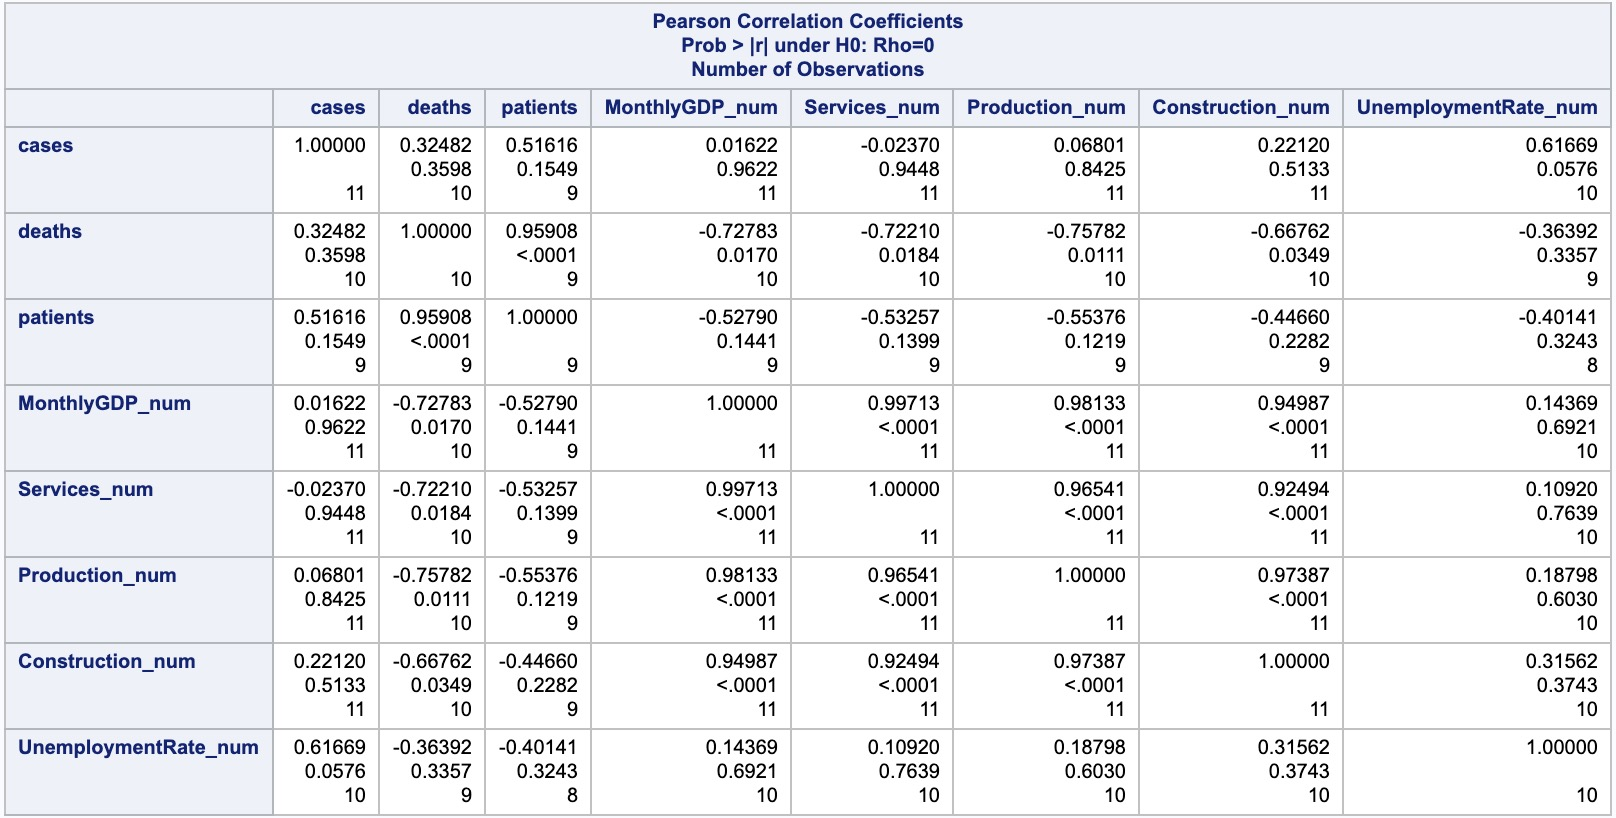
\includegraphics[width=13cm]{corr_economics_new.jpg}
\end{table}

\begin{table}[H]
\centering
\caption{Corrlation Matrix Economics Indicators (cum)}
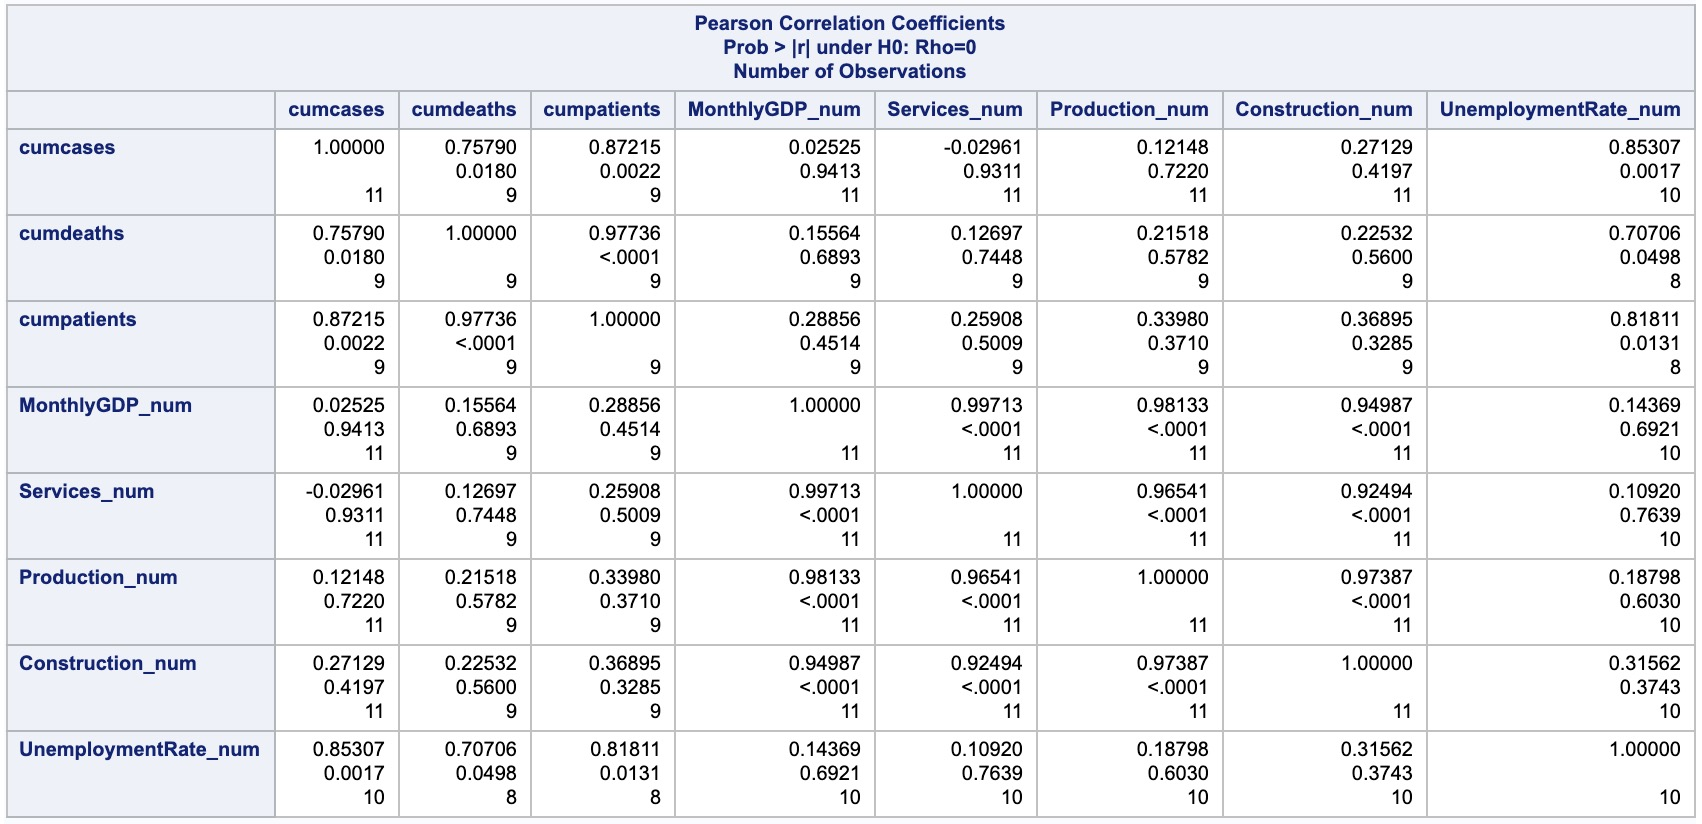
\includegraphics[width=13cm]{corr_economics_cum.jpg}
\end{table}

\begin{table}[H]
\centering
\caption{Correlation Matrix FTSE}
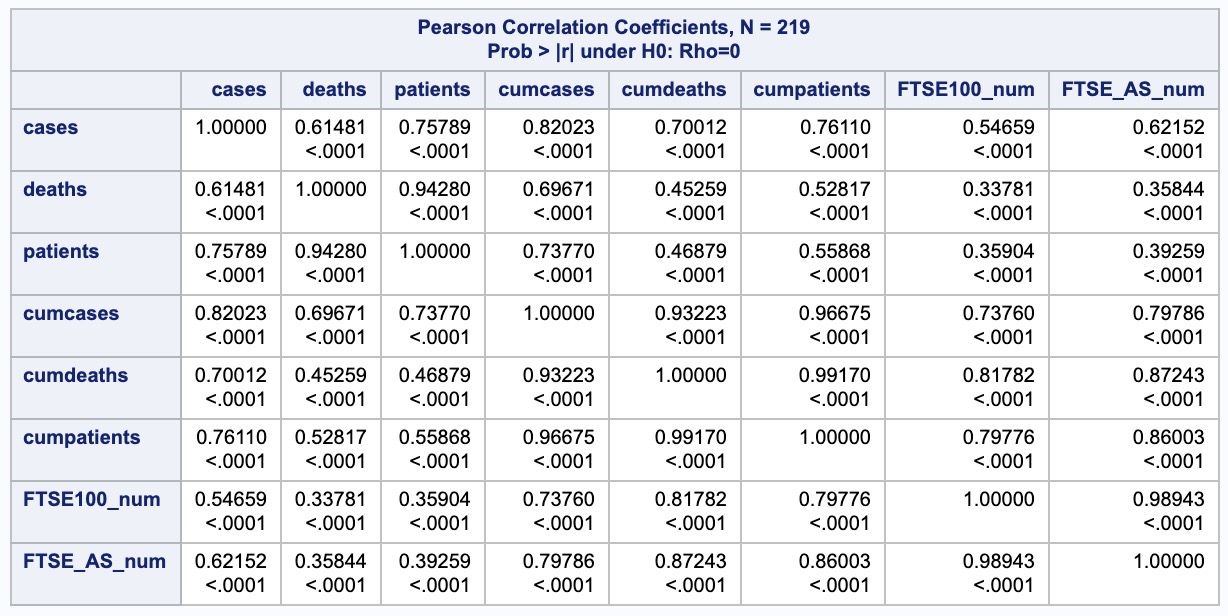
\includegraphics[width=13cm]{corr_stock.jpg}
\end{table}
\hspace*{\fill}

\noindent
2. As for the second question, regression analysis is implemented to further explore how the COVID-19 indicators impact 
the economics indicators. Only highly and significantly correlated variables are chosen to perform regression analysis.
Table 4 and Table 5 is the summary of regression analysis (with only one parameter) on COVID-19 indicators with economics indicators 
and stock indexes, respectively;\par
\noindent

\begin{table}[H]
    \begin{center}
    \caption{Regression Analysis on Economics Indicators}
    \begin{tabular}{llcccc}
        \toprule
        Y&X&Coef&Intercept&p&R-square\\
        \midrule
        Monthly GDP&Deaths&-0.00073&93.31&0.017&0.53\\
        Service Index&Deaths&-0.00068&92.62&0.018&0.52\\
        Production Index&Deaths&-0.00074&96.14&0.011&0.57\\
        Condtruction Index&Deaths&-0.0014&95.28&0.035&0.45\\
        Unemployment Rate&CumCases&1.09e-6&4.05&0.0017&0.73\\
        Unemployment Rate&CumDeaths&2.04e-5&3.73&0.050&0.50\\
        Unemployment Rate&CumCases&7.14e-6&3.62&0.013&0.67\\
        \bottomrule
    \end{tabular}
    \end{center}
\end{table}

\begin{table}[H]
    \begin{center}
    \caption{Regression Analysis on FTSE Indexes}
    \begin{tabular}{llcccc}
        \toprule
        Y&X&Coef&Intercept&p&R-square\\
        \midrule
        FTSE100&CumDeaths&0.0124&5544.47&<0.0001&0.67\\
        FTSE100&CumPatients&0.0031&5626.53&<0.0001&0.64\\
        FTSE100&CumCases&0.00023&5912.69&<0.0001&0.54\\
        FTSE100&cases&0.0112&5976.05&<0.0001&0.30\\
        FTSE All Share&CumDeaths&0.0083&3029.41&<0.0001&0.76\\
        FTSE All Share&CumPatients&0.0021&3080.99&<0.0001&0.74\\
        FTSE All Share&CumCases&0.00016&3274.74&<0.0001&0.64\\
        FTSE All Share&cases&0.0080&3312.77&<0.0001&0.39\\
        \bottomrule
    \end{tabular}
    \end{center}
\end{table}

\section{Conclusion and Limitations}
\textbf{Conclusions:}\par
\noindent
1) Among three newly-added COVID-19 indicators, only the number of deaths has close
relationship with economics indicators and it negatively affects the these indicators.
One additional death case will lead to these indicators decrease 0.00073, 0.00068, 0.0074, and 0.0014.\par
\noindent
2) As for cumulative COVID-19 indicators, all the three indicators only have significant and highly positive correlations
with the unemployment rate. One additional cumulative case, death, patient will lead the unemployment rate to increase 1.09e-6, 2.04e-5, and 7.14e-6, respectively.\par
\noindent
3) All the COVID-19 indicators have significant correlations with two stock indexes. Among these indicators, all the cumulative indicators and 
'cases' indicator have relatively high correlations with stock indexes. One additional cumulative case, death, patient, and newly-added case will lead the 
FTSE 100 index increase 0.0124, 0.0031, 0.00023, and 0.0112, respectively; whereas they will make FTSE All Share index increase 0.0083, 0.0021, 0.00016, and 0.0080, 
respectively.\par

\hspace*{\fill}

\noindent
\textbf{Limitations:}\par
\noindent
1) The number of instances of economics indicators (9 to 11) is relatively limited. More instances will allow us to perform more accurate analysis;\par
\noindent
2) As we can see from the COVID-19 figures above, the COVID-19 crisis in the UK can be divided to three stages. It would be 
better to analyse the correlations between the COVID-19 indicators and stock indexes at different stages;\par
\noindent
3) Although all the simple linear regression models above are significant and have relatively good R-square score, the linear regression itslef may be 
too simple to represent how COVID-19 indicators impact the economics indicators and the stock market exactly.\par


\begin{appendices}
\renewcommand\thefigure{\Alph{section}\arabic{figure}}  
\section{Appendix}
\setcounter{table}{0}
    \begin{table}[H]
        \begin{center}
        \caption{Summary of SAS Steps and Procedures}
        \begin{tabular}{lll}
            \toprule
            Step/Process Name&Macro Name&Used for\\
            proc import&importdata&import raw datasets from csv. or excel files
            \midrule
            FTSE100&CumDeaths&0.0124\\
            FTSE100&CumPatients&0.0031\\
            \bottomrule
        \end{tabular}
        \end{center}
    \end{table}
\end{appendices}
\end{document}